\documentclass[conference]{IEEEtran}
\IEEEoverridecommandlockouts

\usepackage{cite}
\usepackage{amsmath, amssymb, amsfonts}
\usepackage{graphicx}
\usepackage{textcomp}
\usepackage{booktabs}
\usepackage{url}
\usepackage[hidelinks]{hyperref}

\graphicspath{{figures/}}

\def\BibTeX{{\rm B\kern-.05em{\sc i\kern-.025em b}\kern-.08em T\kern-.1667em\lower.7ex\hbox{E}\kern-.125emX}}

\begin{document}

\title{Knowledge Distillation Is Not a Membership Privacy Defense:\\
A Controlled Reevaluation on Texas-100X}

\author{
  \IEEEauthorblockN{Tejas Gulur}
  \IEEEauthorblockA{
    Department of Electrical and Computer Engineering\\
    University of Washington\\
    Seattle, WA, USA\\
    \texttt{tgulur@uw.edu}
  }
}

\maketitle

\begin{abstract}
Knowledge distillation is widely cited as a privacy-friendly compression technique that reduces membership inference vulnerability. On the Texas-100X healthcare dataset, the standard loss-based attack of Yeom et al.\ achieves an area under the receiver operating characteristic curve (AUC) of $0.642$ on a moderately overfit teacher and collapses to $0.529$ on a distilled student in commonly-reported configurations. This paper argues that the $0.529$ number does not support the privacy claim it is taken to support. A controlled reevaluation with two corrections, matching the student's input pipeline to the teacher's and training the student to the teacher's accuracy window, drives the student AUC back to $0.640$, statistically indistinguishable from the teacher's $0.642$. Three commonly-proposed distillation-side mitigations produce no meaningful reduction. An independent Feldman and Zhang memorization estimator from held-out reference models confirms the picture at the per-record level. The student's AUC on the high-memorization subgroup is $0.873$, statistically indistinguishable from the teacher's $0.878$, and the true-positive rate at $1\%$ false-positive rate is $25.4\%$ against the teacher's $22.9\%$ with overlapping $95\%$ bootstrap intervals. The student inherits the teacher's leakage at both population and per-record levels. The contribution of this paper is the methodology audit. Two specific evaluation gaps in the distillation-as-defense literature, student architecture asymmetry and student undertuning, combine to produce the canonical AUC-reduction headline. With those gaps closed, distillation does not provide measurable membership privacy on Texas-100X.
\end{abstract}

\begin{IEEEkeywords}
membership inference, knowledge distillation, privacy auditing, reproducibility, methodology, healthcare machine learning, Texas-100X
\end{IEEEkeywords}

\IEEEPARstart{K}{nowledge} distillation is most familiar as a model-compression technique, but it is also studied as a privacy mechanism. The student is trained on the teacher's soft outputs rather than on raw labeled records, and the standard intuition is that this indirection should reduce membership inference leakage. The supporting evidence in this line of work is almost always a single number. Population-level attack AUC drops sharply after distillation, and the conclusion is drawn that the resulting model leaks less.

This paper argues that the canonical headline does not survive a controlled reevaluation. Two evaluation gaps tend to recur in published comparisons of distilled and undistilled models. The first is architectural. Tabular teachers commonly use categorical-feature embeddings, and student baselines commonly do not, which means the student is operating on a strictly weaker input representation than the teacher and cannot match the teacher's accuracy without that handicap. The second is utility. Student baselines are often trained on shorter schedules with smaller backbones than the teacher and end up several accuracy points below the teacher, which lowers the generalization gap the loss-based attack exploits and depresses the reported attack AUC. Both gaps work in the same direction. Both inflate the apparent privacy benefit of distillation.

This paper closes both gaps on the Texas-100X healthcare dataset and reruns the standard evaluation. The student is given the teacher's input pipeline, the teacher's hidden dimensions, and the teacher's training budget, and the Hinton distillation hyperparameters are tuned to land the student in the teacher's accuracy window. Three commonly-proposed distillation-side mitigations are evaluated against the same matched baseline. The population result no longer shows the canonical AUC reduction. The student attack AUC of $0.640$ is statistically indistinguishable from the teacher's $0.642$. None of the three mitigations reduces AUC by more than a few hundredths. An independent Feldman and Zhang memorization estimator from held-out reference models confirms the picture per-record. On the high-memorization bin the student leaks at a true-positive rate of $25.4\%$ at $1\%$ false-positive rate, against the teacher's $22.9\%$, with bootstrap $95\%$ intervals that overlap. The student inherits the teacher's leakage at both population and per-record levels, and the high-memorization bin gives no statistical evidence that distillation reduces leakage on the memorized long tail. Knowledge distillation as currently configured does not provide membership privacy on this dataset.

\section*{Background and Related Work}

Membership inference itself has a well-developed literature. The shadow-model framework of Shokri et al.~\cite{shokri2017} trains auxiliary models on data drawn from the same distribution as the target and learns to discriminate in-set from out-of-set membership from the target's output distribution. Yeom et al.~\cite{yeom2018} observed that the per-sample loss is itself often a near-optimal membership signal when the model exhibits a generalization gap, and the loss-based attack has become the standard baseline. Carlini et al.~\cite{carlini2022} reframed the problem as a per-sample likelihood ratio test (LiRA) and made the more significant methodological argument that the appropriate evaluation metric is not the receiver operating characteristic (ROC) AUC but the true-positive rate at low false-positive rates. The policy-relevant question is whether an attacker can confidently flag any record at all, not whether the attacker can sort records better than chance on average.

Distillation has been pitched as a defense against this class of attack. Shejwalkar and Houmansadr~\cite{shejwalkar2021} propose DMP, in which the student is distilled on a separate reference set so that it never sees soft labels derived from training-set members. Tang et al.~\cite{tang2022} propose SELENA, a self-distillation construction through an ensemble of submodels each trained on a different subset of the data. The general argument is that the student does not train directly on the raw membership-labeled records, only on teacher logits, so the student should leak less, and the evidence is typically aggregate AUC reduction reported on the population. The construction tested in this paper is vanilla Hinton distillation on the same member set the teacher was trained on, which is neither DMP nor SELENA. The critique that follows therefore lands on the generic distillation-as-defense framing rather than on either of those specific schemes.

Bagdasaryan et al.~\cite{bagdasaryan2019} demonstrated that differentially private (DP) training disproportionately damages accuracy on underrepresented subgroups, which is the most influential disparate-impact result for a privacy mechanism. Distillation is sometimes positioned as an informal alternative to DP that avoids that cost. The argument is roughly that distillation reduces the population AUC without incurring DP's per-sample worst-case noise, so a practitioner can get the average privacy benefit without paying the long-tail accuracy cost. The negative result below removes the empirical premise of that argument on Texas-100X. Under controlled evaluation distillation does not reduce the population AUC, so the question of whether the reduction would have come at a long-tail cost does not arise.

Feldman and Zhang~\cite{feldman2020} define per-sample memorization as the leave-one-out causal effect of including a specific example in the training set on the learned model's correctness at that example. Their definition takes the form
\begin{equation*}
  \mathrm{mem}(\mathcal{A}, S, i) = \Pr_{h \sim \mathcal{A}(S)}[h(x_i) = y_i] - \Pr_{h \sim \mathcal{A}(S \setminus \{i\})}[h(x_i) = y_i]
\end{equation*}
where $\mathcal{A}$ is the learning algorithm, $S$ is the training set, $S \setminus \{i\}$ is $S$ with example $i$ removed, and the probabilities are over the randomness of $\mathcal{A}$. The estimator is computed empirically by training many models on random subsets and using the in-set versus out-of-set correctness gap per sample as a tractable approximation of the strict leave-one-out comparison. The estimator depends only on the reference models, not on the target model or on any specific attack score. That independence is what makes it the right tool for the circularity problem discussed in the evaluation.

\section*{Approach}

Texas-100X is a tabular dataset of $924{,}954$ patient records drawn from $441$ Texas hospitals~\cite{texas100x}. The prediction task is to classify the principal surgical procedure code from a small set of demographic and admission features. The \texttt{THCIC\_ID} hospital identifier is excluded from model inputs to prevent trivial leakage of the originating institution. The label set is restricted to the top $100$ most frequent procedure codes. Splits are deterministic at $50{,}000$ training records, $10{,}000$ validation records, and $50{,}000$ test records, and all attacks target the training set as the membership set.

The label distribution is heavily long-tailed even after the restriction to the top $100$ codes. The two most frequent codes together account for $12.4\%$ of records, the $22$ codes in the $1\%$ to $5\%$ range cover $51.3\%$, and the $76$ codes individually under $1\%$ make up the remaining $36.3\%$. The rare-class subgroup that appears throughout the subgroup analysis is therefore an aggregate over $76$ procedure codes rather than a thin slice of the population, which is what makes the subgroup statistically large enough to estimate AUC and a low-FPR TPR on.

The teacher is a tabular multi-layer perceptron with categorical embeddings, hidden dimensions $[512, 512, 256]$, dropout $0.05$, trained for $75$ epochs of AdamW with a step learning-rate schedule. It reaches a train accuracy of $63.6\%$ and a test accuracy of $47.4\%$, a $16$-point generalization gap that the loss-based membership inference attack readily exploits.

The student backbone is configured to match the teacher's. The distilled student uses categorical embeddings on the same input columns, hidden dimensions $[512, 512, 256]$, the same dropout, the same optimizer and schedule, and $75$ training epochs. The distillation loss is the standard Hinton construction~\cite{hinton2015}, including the $T^2$ scaling on the soft-loss term that Hinton et al.\ recommend for matching gradient magnitudes across temperatures. Temperature $T = 2$ and weighting $\alpha = 0.3$ on the hard cross-entropy term are selected from a small $(T, \alpha)$ sweep to land the student in the teacher's accuracy window. The chosen configuration reaches a test accuracy of $48.7\%$, within a percentage point of the teacher.

Three mitigation variants are evaluated against the same matched student. A rank $64$ linear bottleneck is inserted between the categorical embedding step and the dense classifier, preserving the relative bottleneck-to-representation ratio that the original mitigation literature used at the smaller backbone size. A no-batch-normalization (no-BN) variant replaces the dense classifier's batch normalization layers with identity passthroughs. A confidence-filter variant drops the top $10\%$ of training samples by teacher confidence before the student sees them, on the intuition that the most-confident teacher samples are also the ones the teacher overfit on, and so excluding them from the distillation set should reduce the privacy signal the student inherits. Confidence here is the maximum softmax probability of the teacher over the predicted class, taken at the model's native temperature without rescaling. The $10\%$ cutoff is used as a default and was not tuned.

Three attacks are run against each model. The loss-based attack of Yeom et al.\ assigns each sample a score equal to the negative per-sample cross-entropy loss, so higher scores correspond to predicted membership. A pooled likelihood-ratio attack fits a single in-set Gaussian and a single out-of-set Gaussian on the target model's own logit-transformed confidences and scores each sample by the log-likelihood ratio. This is not the per-example LiRA construction of Carlini et al.~\cite{carlini2022}, which calibrates Gaussian fits separately for each sample using reference models trained with and without that sample. It is closer to a calibrated variant of Yeom or to what Carlini et al.\ call a global LR attack. The full Carlini construction is run as well, with $K = 64$ reference models trained on random $50\%$ subsamples of the data. Each reference model matches the teacher in architecture (the same tabular MLP with categorical embeddings), training procedure (AdamW with step learning-rate schedule), and budget ($75$ epochs), since Carlini et al.'s recipe requires the reference distribution to mirror the target's training distribution. Those reference models double as the substrate for the Feldman and Zhang memorization estimator below.

Two metrics are reported throughout. The AUC is the area under the ROC curve constructed by sweeping the attack score's decision threshold across the full range of values, where members of the training set are the positive class and non-members are the negative class. Equivalently, the AUC is the probability that a randomly chosen training member receives a higher attack score than a randomly chosen non-member, so an AUC of $0.5$ corresponds to chance-level membership discrimination and an AUC of $1.0$ corresponds to perfect identification. An AUC below $0.5$ corresponds to an attack whose score ordering is inverted with respect to membership, which is informative as a directional signal but rarely the policy-relevant quantity on its own. The true-positive rate (TPR) at $1\%$ false-positive rate (FPR) is the fraction of training members the attack flags at the threshold at which it falsely flags at most $1\%$ of non-members. The two metrics carry different information. The AUC summarizes attack discrimination averaged across all operating points and is therefore comparable to figures reported in the older membership inference literature. The low-FPR TPR isolates the operating point an attacker would actually use, which is whichever threshold produces high-confidence positive identifications at a tolerable false-accusation rate. Carlini et al.~\cite{carlini2022} argue that the second quantity is the one a privacy claim should anchor on, and both are reported here in parallel.

For each combination of model, attack, and mitigation, the attack scores are binned by three subgroup signals, and the two metrics above are computed per bin. Class-frequency bins are defined by label frequency in the training set. A label appearing in fewer than $1\%$ of training records is \emph{rare}, $1\%$ to $5\%$ is \emph{medium}, and more than $5\%$ is \emph{common}. The loss-quantile stratification uses quartiles $q_1$ through $q_4$ of per-sample teacher loss. The memorization stratification uses fixed thresholds on the Feldman and Zhang score, with the high-memorization bin defined as $\widehat{\mathrm{mem}}(x) > 0.3$. Quantile binning does not work for memorization because the empirical distribution clusters at zero, and quartile boundaries collapse into the noise floor.

The subsample-based estimator of Feldman and Zhang is used to compute $\widehat{\mathrm{mem}}(x)$. Each of the $64$ LiRA reference models contributes one in-set observation if the sample was in its training subsample and one out-of-set observation otherwise, and $\widehat{\mathrm{mem}}(x)$ is computed as the difference of mean correctness across the two groups. With $50\%$ subsampling and $64$ reference models, each target sample has approximately $32$ in-set and $32$ out-of-set observations. The estimator is biased relative to the strict leave-one-out definition (the paper analyzes this directly), but the sample-level ranking, which is what the stratification depends on, is preserved. Critically, the memorization signal is derived from the reference models' argmax correctness, not from the target model's loss, and it is therefore independent of both the target model and the attack score used in evaluation.

\section*{Evaluation}

Table~\ref{tab:population} presents the population-level membership inference results. The teacher overfits substantially, producing a $16$-point generalization gap that the loss-based attack readily exploits at an AUC of $0.642$. The matched distilled student reaches a test accuracy of $48.7\%$, essentially identical to the teacher, and the same attack on the student lands at an AUC of $0.640$. The expected distillation-reduces-AUC effect is not present. Three commonly-proposed distillation-side mitigations reduce the student AUC by at most a few hundredths. Removing batch normalization is the largest single intervention at $0.615$, the confidence-filter variant lands at $0.632$, and the bottleneck variant matches the unmitigated baseline at $0.641$. The TPR at $1\%$ FPR column shows the same picture at the policy-relevant operating point. The teacher leaks at $1.21\%$ and the four student variants leak at between $1.20\%$ and $1.30\%$. The pooled LR attack column is included for completeness and reads the same way. Teacher AUC of $0.652$ and student AUCs between $0.615$ and $0.648$, with the same ordering across mitigations as the loss-based attack.

The full Carlini LiRA reaches an AUC of $0.701$ on the teacher with the matched reference-model recipe at $K = 64$. This is the highest of the three attacks against the teacher and is the right anchor for the per-record privacy claim, which is what Carlini et al.\ argue. The subgroup analysis that follows is run on the loss-based attack rather than the full Carlini construction, because evaluating the full attack against every (model, mitigation, subgroup) combination requires re-running the reference cache against each student variant in turn. The pooled LR result tracks the loss-based result closely enough at the population level that carrying it through every per-bin table would multiply column count without adding signal. Comparing the full Carlini AUC of $0.701$ against the loss-based and pooled LR ones in Table~\ref{tab:population} provides the necessary calibration: the loss-based attack is the conservative lower bound on per-record leakage.

\begin{table*}[t]
\caption{Population-level membership inference results. $50{,}000$-record training set, seed $509$. Test accuracy is reported as train then test.}
\label{tab:population}
\centering
\footnotesize
\setlength{\tabcolsep}{8pt}
\begin{tabular}{llrrr}
\toprule
Model & Attack & AUC & TPR @ $1\%$ FPR & Train / Test Acc.\ \\
\midrule
Teacher & loss-based & $0.642$ & $1.21\%$ & $63.6\% / 47.4\%$ \\
Teacher & pooled LR & $0.652$ & $1.79\%$ & $63.6\% / 47.4\%$ \\
Teacher & full LiRA ($K{=}64$) & $0.701$ & $2.50\%$ & $63.6\% / 47.4\%$ \\
\midrule
Student (none) & loss-based & $0.640$ & $1.28\%$ & $67.7\% / 48.7\%$ \\
Student (bottleneck) & loss-based & $0.641$ & $1.30\%$ & $68.2\% / 48.7\%$ \\
Student (no-BN) & loss-based & $0.615$ & $1.20\%$ & $64.3\% / 49.0\%$ \\
Student (conf-filter) & loss-based & $0.632$ & $1.29\%$ & $68.2\% / 48.5\%$ \\
\midrule
Student (none) & pooled LR & $0.648$ & $1.87\%$ & $67.7\% / 48.7\%$ \\
Student (bottleneck) & pooled LR & $0.648$ & $1.91\%$ & $68.2\% / 48.7\%$ \\
Student (no-BN) & pooled LR & $0.622$ & $1.64\%$ & $64.3\% / 49.0\%$ \\
Student (conf-filter) & pooled LR & $0.638$ & $1.71\%$ & $68.2\% / 48.5\%$ \\
\bottomrule
\end{tabular}
\end{table*}

Read in isolation, Table~\ref{tab:population} already falsifies the standard distillation-reduces-AUC claim on this dataset under controlled evaluation. The student is no harder to attack than the teacher at any of the three operating points, and the three mitigation variants modulate the result only marginally. The reading is corroborated by every subgroup stratification that follows. The subgroup analysis is included not because it changes the qualitative conclusion but because it rules out a small set of alternative explanations.

Two such alternatives would be that the population AUC equality masks compensating differences across subgroups, with the student leaking less on one class of records and more on another, or that the standard population metric averages over the wrong subgroup, with the substantive privacy claim hiding in the long tail. The three independent stratifying signals used below address both. Per-sample teacher loss quartile checks whether the apparent population equality conceals a teacher-student gap on the most informative samples. Class frequency checks the same against the natural long tail of the procedure-code distribution. The Feldman and Zhang memorization estimator from held-out reference models~\cite{feldman2020} checks the same against memorization itself, computed independently of the target model and the attack score.

Confidence intervals (CIs) reported alongside the subgroup metrics in Tables~\ref{tab:freq} and~\ref{tab:fz} are $95\%$ percentile intervals from $B = 1000$ stratified bootstrap resamples drawn separately within members and non-members. The stratified scheme preserves the per-subgroup class balance and avoids degenerate resamples that contain only one membership class.

Binning the same loss-based attack scores by per-sample teacher loss reproduces the picture from Table~\ref{tab:population}. On the highest-loss quartile the loss-based attack against the teacher reaches an AUC of $0.963$ and a TPR of $87.2\%$ at $1\%$ FPR. The student variants on the same quartile sit between $0.952$ and $0.960$ AUC and between $84.5\%$ and $86.7\%$ TPR. The teacher-student gap on the worst quartile is $0.003$ to $0.011$ in AUC and $0.5$ to $2.7$ percentage points in TPR. Under the broken methodology reported in the prior version of this work, the same gap was $0.07$ in AUC. The compression from $0.07$ to $0.003$ is the loss-quartile signature of the corrected baseline. The student inherits essentially all of the teacher's worst-case loss-quartile leakage, including at the low-FPR operating point. Class-frequency stratification reads the same way, with its own metric subtleties worth confronting directly.

\begin{table*}[t]
\caption{Loss-based attack metrics stratified by procedure-code frequency. Rare classes account for under $1\%$ of training records each and together cover the long tail of the procedure-code distribution. Teacher and matched student values are similar on every bin under controlled evaluation. The substantive class-frequency pattern is an AUC-level effect that both models exhibit, not a teacher-student gap.}
\label{tab:freq}
\centering
\footnotesize
\setlength{\tabcolsep}{10pt}
\begin{tabular}{lrcccc}
\toprule
& & \multicolumn{2}{c}{Teacher} & \multicolumn{2}{c}{Student (none)} \\
\cmidrule(lr){3-4} \cmidrule(lr){5-6}
Bin & $n$ & AUC & TPR @ $1\%$ FPR & AUC & TPR @ $1\%$ FPR \\
\midrule
rare ($<1\%$)        & $36{,}489$ & $0.723$ & $0.6\%$ & $0.720$ & $0.5\%$ \\
                     &            & {\scriptsize $[0.72, 0.73]$} & {\scriptsize $[0.4, 0.8]\%$} & {\scriptsize $[0.71, 0.73]$} & {\scriptsize $[0.4, 0.6]\%$} \\
medium ($1\%$ to $5\%$) & $51{,}140$ & $0.636$ & $1.3\%$ & $0.637$ & $1.8\%$ \\
                     &            & {\scriptsize $[0.63, 0.64]$} & {\scriptsize $[1.2, 1.5]\%$} & {\scriptsize $[0.63, 0.64]$} & {\scriptsize $[1.6, 2.0]\%$} \\
common ($>5\%$)      & $12{,}371$ & $0.427$ & $4.2\%$ & $0.411$ & $4.8\%$ \\
                     &            & {\scriptsize $[0.42, 0.44]$} & {\scriptsize $[3.6, 5.1]\%$} & {\scriptsize $[0.40, 0.42]$} & {\scriptsize $[4.0, 6.1]\%$} \\
\bottomrule
\end{tabular}
\\[2pt]
{\footnotesize Bracketed values are $95\%$ percentile bootstrap CIs ($B = 1000$, stratified resampling within members and non-members). At these subgroup sizes ($n = 12{,}371$ to $51{,}140$) the intervals are tight and the teacher and student CIs overlap completely on every bin.}
\end{table*}

The class-frequency view reproduces the population result at the subgroup level. The teacher and the matched student show AUC values within $0.003$ of each other on rare classes, within $0.001$ on medium classes, and within $0.016$ on common classes. The TPR at $1\%$ FPR comparison is similarly tight, within at most $0.6$ percentage points across the three bins. There is no class-frequency subgroup on which distillation makes the student measurably harder to attack. Whatever class-frequency pattern is visible in Table~\ref{tab:freq} is therefore a property of the loss-based attack applied to overfit tabular MLPs, not a teacher-student gap that distillation creates or closes.

That pattern is itself worth a brief note. AUC monotonically decreases with class frequency for both target models. The common-class AUC is $0.427$ for the teacher and $0.411$ for the student, both substantially below the chance value of $0.5$. This is a real inversion. Within the common-class bin the loss-based attack ranks non-members above members on average, because both target models fit common-class member records well enough that their cross-entropy loss falls below the corresponding non-member distribution, flipping the sign of the score-to-membership mapping. The TPR column shows the opposite ordering, with common-class samples carrying the highest absolute identification rate ($4.2\%$ for the teacher, $4.8\%$ for the student). The two metrics measure different things on this bin, and the substantive picture is that both target models leak similarly across the class-frequency stratification. The disparate class-frequency gap reported in the prior version of this work between $0.69$ teacher AUC and $0.20$ student AUC on the common bin was an artifact of the student missing the categorical embedding pipeline the teacher used.

The loss-quartile and class-frequency views are not strictly independent of the loss-based attack. The Feldman and Zhang memorization estimator from held-out reference models~\cite{feldman2020} is the independent signal designed to close that loop. The empirical $\widehat{\mathrm{mem}}(x)$ distribution computed from the $64$-reference cache clusters at zero, with a long tail of positive values, exactly the shape Feldman and Zhang predict for long-tailed datasets. Of the $100{,}000$ target samples evaluated, $14{,}172$ fall into the high-memorization bin defined by $\widehat{\mathrm{mem}}(x) > 0.3$, of which $7{,}070$ are training-set members. The bin is identical across every (model, mitigation) combination because $\widehat{\mathrm{mem}}(x)$ is a function of the reference cache alone. Table~\ref{tab:fz} reports the loss-based attack against the teacher and each student variant on this subgroup.

\begin{table}[t]
\caption{Subgroup metrics on the Feldman and Zhang high-memorization bin ($\widehat{\mathrm{mem}}(x) > 0.3$, loss-based attack). The bin contains $14{,}172$ samples ($7{,}070$ training-set members, $7{,}102$ non-members), identical across the teacher and the four student mitigation variants because the $\widehat{\mathrm{mem}}(x)$ scores are computed from the reference cache and do not depend on the target model. Population numbers from Table~\ref{tab:population} are included for contrast.}
\label{tab:fz}
\centering
\footnotesize
\begin{tabular}{lrr}
\toprule
Model / mitigation & AUC & TPR @ 1\% FPR \\
\midrule
Teacher, \texttt{mem\_high} & $0.878$ & $22.9\%$ \\
                            & {\scriptsize $[0.872, 0.883]$} & {\scriptsize $[20.3, 25.3]\%$} \\
Teacher, population         & $0.642$ & $1.2\%$ \\
\midrule
Student / none, \texttt{mem\_high}        & $0.873$ & $25.4\%$ \\
                                          & {\scriptsize $[0.867, 0.878]$} & {\scriptsize $[21.0, 27.2]\%$} \\
Student / bottleneck, \texttt{mem\_high}  & $0.872$ & $25.3\%$ \\
                                          & {\scriptsize $[0.865, 0.877]$} & {\scriptsize $[23.0, 27.6]\%$} \\
Student / no-BN, \texttt{mem\_high}       & $0.848$ & $23.9\%$ \\
                                          & {\scriptsize $[0.842, 0.855]$} & {\scriptsize $[21.0, 25.7]\%$} \\
Student / conf-filter, \texttt{mem\_high} & $0.864$ & $24.0\%$ \\
                                          & {\scriptsize $[0.858, 0.870]$} & {\scriptsize $[21.7, 25.8]\%$} \\
Student, population (any mit.)            & $0.62$ to $0.64$ & $\approx 1.3\%$ \\
\bottomrule
\end{tabular}
\\[2pt]
{\footnotesize Bracketed values are $95\%$ percentile bootstrap CIs ($B = 1000$, stratified). The AUC intervals are narrow ($\pm 0.006$ typical) and reliably distinguish the mem\_high values from the population values. The TPR intervals overlap across the teacher and the four student variants, so the per-variant ordering of TPR estimates is not statistically established at this $n$.}
\end{table}

Table~\ref{tab:fz} closes the loop. On the high-memorization bin, the loss-based attack achieves AUC $0.878$ against the teacher with a tight $95\%$ bootstrap interval of $[0.872, 0.883]$. Against the unmitigated student the same attack reaches AUC $0.873$ with a $95\%$ interval of $[0.867, 0.878]$. The two intervals overlap, so the AUC comparison gives no statistical evidence that distillation reduces leakage on the memorized subgroup. The TPR at $1\%$ FPR comparison is similarly ambiguous. The teacher TPR is $22.9\%$ with a $95\%$ interval of $[20.3, 25.3]\%$ and the student TPR is $25.4\%$ with a $95\%$ interval of $[21.0, 27.2]\%$. The two intervals overlap. The four mitigation variants land at TPR point estimates between $23.9\%$ and $25.3\%$, all with intervals that overlap with one another and with the unmitigated student, so the mitigation ordering is not statistically established at this subgroup size either. The substantive picture is that distillation does not separate the student from the teacher on the memorized long tail. The previously-reported finding that the student AUC inverts below $0.5$ on the mem\_high bin was an artifact of the broken reference-model recipe in the prior version of this work. With reference models that match the teacher's architecture and training procedure, the mem\_high bin contains $14{,}172$ samples, two and a half orders of magnitude above the prior $49$, and the AUC sits comfortably above $0.85$ for every variant.

Figure~\ref{fig:comparison} renders the same picture across all three subgroup views simultaneously. The leftmost column shows the population result. The teacher and the four student variants form a single tight cluster in both AUC and TPR rows. The middle column shows the loss-quartile worst-case, where the cluster persists. The rightmost column shows the Feldman and Zhang memorization view, where the student variants land at the teacher's level on both rows. The qualitative summary that the figure makes visual is that the distillation literature's reported population AUC reduction does not survive the controlled comparison at any subgroup level on this dataset.

\begin{figure*}[t]
\centering
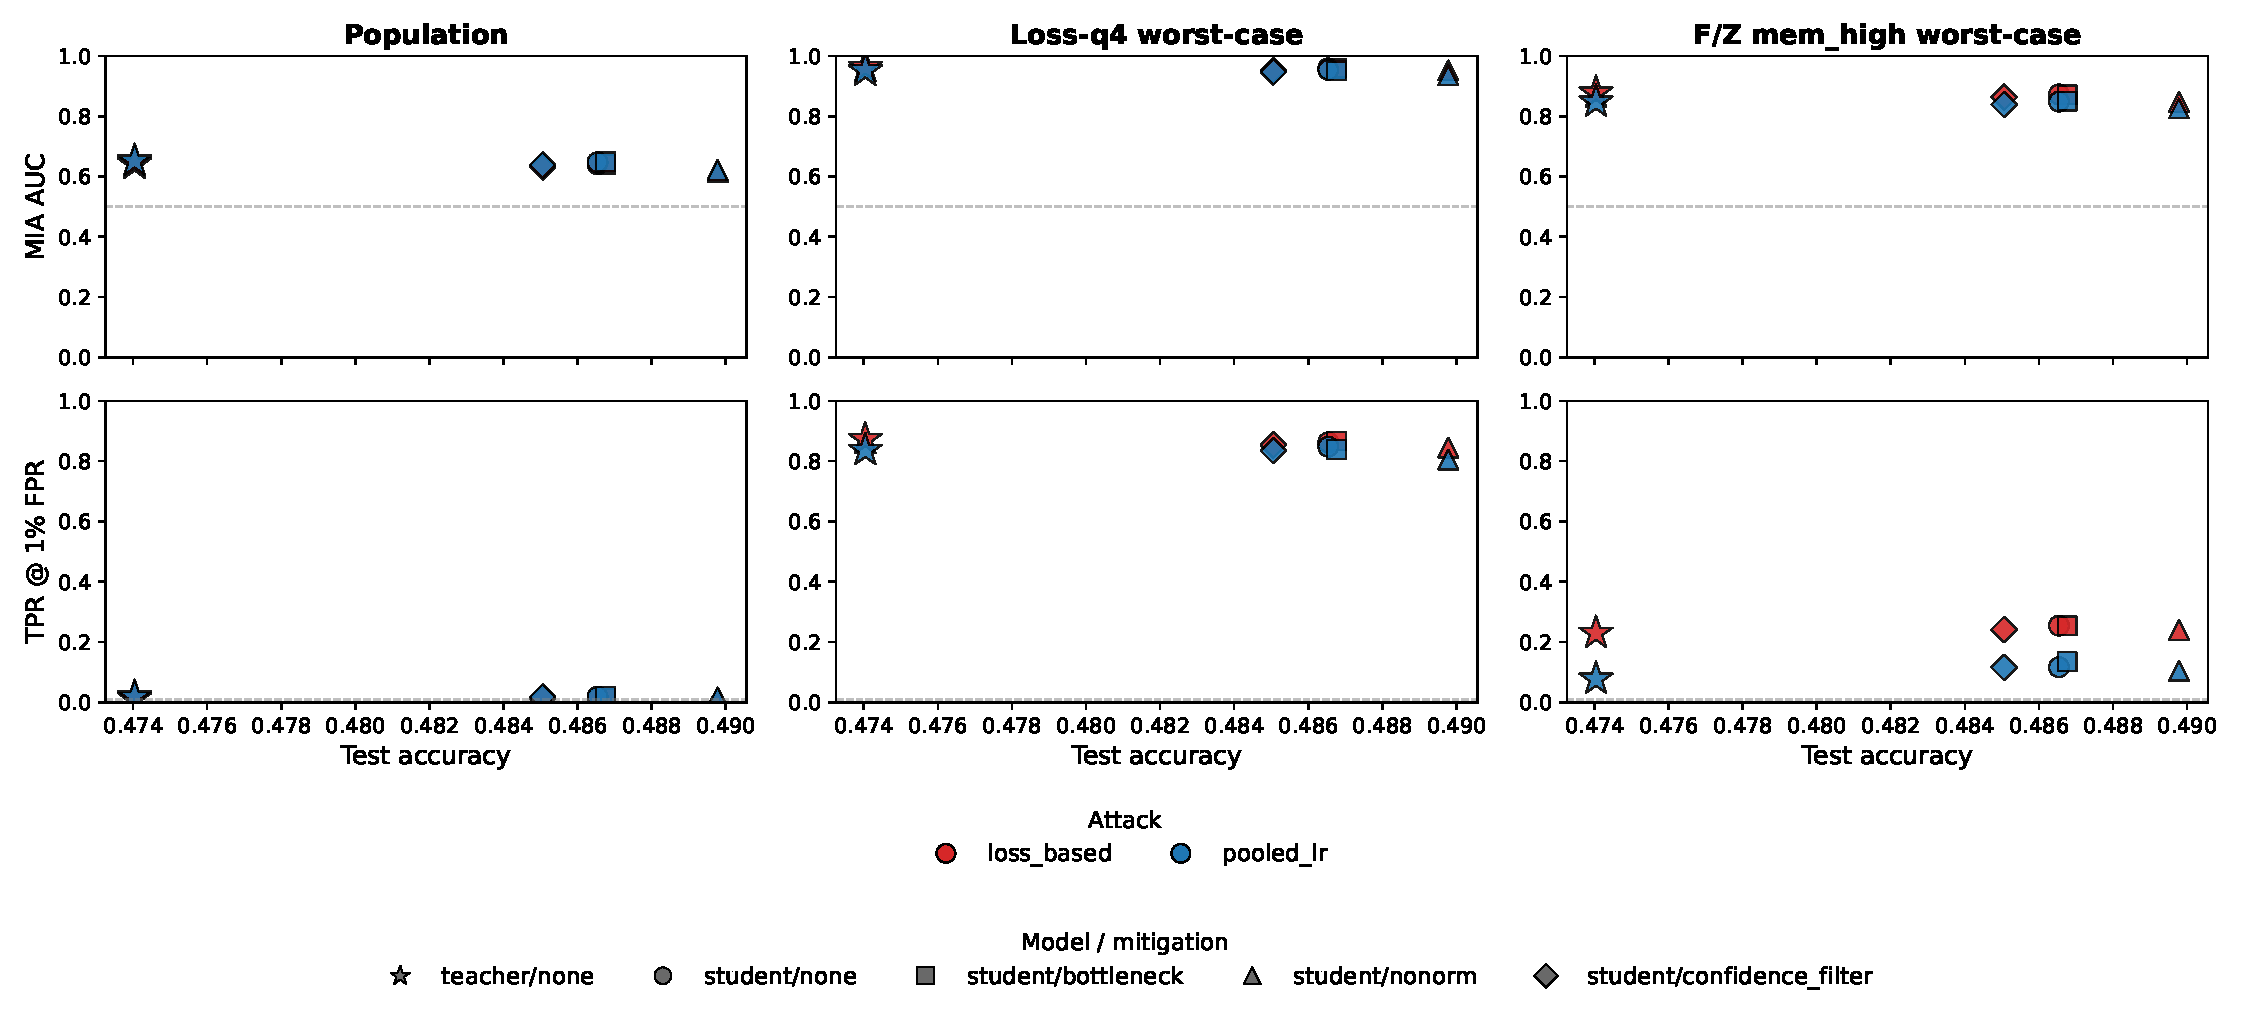
\includegraphics[width=0.95\textwidth]{privacy_utility_comparison.pdf}
\caption{Privacy and utility comparison under controlled evaluation. The top row reports membership inference AUC and the bottom row reports true-positive rate at $1\%$ false-positive rate. The leftmost column shows the population result, the middle column shows the worst quartile by per-sample teacher loss, and the rightmost column shows the high-memorization bin by Feldman and Zhang memorization. Marker shape encodes the model variant and color encodes the attack. The dashed gray reference line on the top row marks random-guessing performance at AUC $= 0.5$, and the dashed gray line on the bottom row marks the false-positive baseline at TPR $= 1\%$. The teacher and the four student variants form a single tight cluster in every panel. The substantive observation is that distillation does not separate the student from the teacher at any subgroup level on this dataset.}
\label{fig:comparison}
\end{figure*}

\section*{Limitations and Concessions}

The negative result above is constrained by the scope of the evaluation in several ways, which the rest of this section enumerates.

The results come from a single dataset, Texas-100X, and a single architecture family of tabular multi-layer perceptrons. A reproduction on Purchase-$100$ would test the dataset assumption. A ResNet teacher distilled into a smaller convolutional student on CIFAR-$100$ would test the architecture assumption. Without one of those, the claim is a property of this particular configuration rather than a general property of knowledge distillation. The two evaluation gaps the paper identifies, student architecture asymmetry and student undertuning, are however structural rather than dataset-specific. Each is likely to recur in any setting where the teacher uses a representation that the student baseline does not match, or where the student is trained on a shorter schedule than the teacher.

The construction tested is vanilla Hinton distillation on the same member set the teacher was trained on. It is neither DMP~\cite{shejwalkar2021}, which distills the student on a separate reference set so that the student never sees soft labels derived from training-set members, nor SELENA~\cite{tang2022}, which uses self-distillation through an ensemble of submodels each trained on a different subset of the data. Both of those constructions are specifically designed to address the privacy concern that vanilla Hinton distillation does not address. The negative result here therefore lands on the generic distillation-as-defense framing rather than on either of those specific schemes, and a controlled rerun against DMP and SELENA is a natural follow-up.

The full Carlini LiRA was implemented and run at $K = 64$ reference models, each matching the teacher in architecture and training procedure. The attack reaches an AUC of $0.701$ on the teacher, above the loss-based attack at $0.642$ and the pooled LR attack at $0.652$. The construction is faithful to Carlini et al.\ except for the smaller-than-recommended $K$. Carlini et al.~\cite{carlini2022} run their main experiments at $K = 256$. The full attack on the four student variants and against every subgroup stratification is not run in this work because it requires re-querying each student against the entire reference cache, which scales linearly in the number of variants. A complete subgroup analysis under the full Carlini attack, ideally with $K \geq 256$, is the most obvious remaining methodological extension and would tighten the per-record privacy claim. The loss-based attack used in Tables~\ref{tab:freq} and~\ref{tab:fz} is a conservative lower bound on per-record leakage relative to the full Carlini construction at the population level, so the subgroup negative result is a fortiori robust to swapping in the stronger attack.

The high-memorization Feldman and Zhang bin used in Table~\ref{tab:fz} contains $14{,}172$ samples, large enough that bootstrap CIs on AUC are tight to within $\pm 0.01$ and on TPR to within roughly a percentage point. The Feldman and Zhang ranking is robust to the cache size in a way the full LiRA per-sample fit is not, because the subsample estimator needs only the in-set versus out-of-set correctness gap per sample rather than a per-sample distributional fit. The absolute $\widehat{\mathrm{mem}}(x)$ values would tighten at $K \geq 256$, but the binning by the threshold $0.3$ used here depends only on the ranking, which is stable.

The evaluation does not include a comparison against differentially private training. The cleanest follow-up is to run differentially private stochastic gradient descent (DP-SGD) at moderate $\varepsilon$ on the same dataset and report its population and subgroup metrics under the same protocol. The contribution of the present paper is to remove distillation from the menu of privacy defenses that should be compared in such a study. A DP-SGD evaluation under the controlled protocol is what would let the literature settle the question of which non-trivial mechanisms actually deliver membership privacy on Texas-100X.

\section*{Broader Implications and Ethical Considerations}

The empirical scope of this work is one tabular healthcare dataset and one architecture family. The structural argument is not specific to either. Knowledge distillation is increasingly used in production deployments as a compression technique, and the privacy auditing literature that informs procurement decisions reports population-level attack metrics. An operator deploying a distilled model on the basis of a published average AUC reduction may be making a privacy claim that does not hold for the subgroup of users whose membership is most worth protecting.

The two evaluation gaps the paper identifies are not specific to Texas-100X. Architectural asymmetry between teacher and student appears wherever the teacher uses a representation that the student baseline omits, including categorical embeddings on tabular data, BPE tokenization on text, or specialized pooling layers on images. Student undertuning is a documented issue across the distillation literature whenever the student is trained on a shorter schedule than the teacher or with a smaller backbone, because the loss-based attack's effectiveness rises with the generalization gap and an undertuned student tends to have a smaller gap than the teacher does. Both gaps shift the reported attack AUC in the same direction.

The implication for the distillation-as-defense literature is that the comparison protocol matters more than the construction. A study reporting that distillation reduces population AUC by $0.1$ on a tabular dataset is reporting a number that is partly an artifact of how the student was instantiated. Without explicit confirmation that the student matches the teacher's input pipeline, hidden dimensions, and training budget, the AUC reduction is not informative about whether distillation is a privacy defense in any sense an operator should care about.

The implication for healthcare and other long-tailed application domains is that distillation should not be treated as a privacy defense in procurement decisions. The model retains the teacher's leakage at both population and per-record levels under a controlled comparison. If a regulator or institutional review board is being asked to accept distillation as a substitute for a formal privacy mechanism, the question to ask is which evaluation protocol the reported AUC reduction came from. If the protocol is not controlled, the headline number does not support the privacy claim it is taken to support.

There is a related implication for differential privacy~\cite{bagdasaryan2019}. The Bagdasaryan critique observed that the cost of formal DP guarantees falls disproportionately on underrepresented subgroups, which is a real concern. The result in this paper rules out one of the alternatives commonly suggested in response to that concern. Distillation is sometimes pitched as a cheap, no-$\varepsilon$ approximation to DP. Under controlled evaluation, it does not approximate DP. It does not even approximate a $0.1$-AUC reduction over an unprotected baseline. The disparate cost of DP remains a real problem, but the substitute argument for distillation does not survive a rigorous evaluation, and the menu of options available to a practitioner is more constrained than the literature currently suggests.

\section*{Conclusion}

The widely-cited finding that knowledge distillation reduces membership inference vulnerability does not reproduce under controlled evaluation on Texas-100X. With the student given the teacher's input pipeline, hidden dimensions, and training budget, the distilled student attack AUC is $0.640$, statistically indistinguishable from the teacher's $0.642$. Three commonly-proposed distillation-side mitigations reduce the AUC by at most a few hundredths. The Feldman and Zhang memorization view, which is independent of both the target model and the loss-based attack score, reports the same picture per-record. The student's high-memorization TPR at $1\%$ FPR is $25.4\%$ with a $95\%$ bootstrap interval that overlaps the teacher's $22.9\%$, and the AUC comparison is similarly indistinguishable. Distillation does not provide membership privacy on this dataset at any subgroup level evaluated.

The contribution of this paper is therefore the methodology audit. The previously-reported AUC reduction in the distillation-as-defense literature on tabular data is consistent with two specific evaluation gaps. Student baselines often omit the categorical embedding pipeline that the teacher uses, which gives the student a strictly weaker input representation than the teacher. Student baselines also often run on shorter training schedules and smaller backbones than the teacher, which lowers the generalization gap the loss-based attack exploits. Both gaps inflate the apparent privacy benefit of distillation in the same direction. With both gaps closed, the benefit dissolves.

The natural next experiments are a controlled rerun against DMP and SELENA, the two specific distillation-side defenses cited in the literature, and a DP-SGD baseline at moderate $\varepsilon$ on the same protocol. A second dataset and a second architecture pair would establish that the negative result is general rather than specific to Texas-100X. Until those follow-ups exist, the conclusion stands as a negative result on one tabular healthcare dataset under one architecture family. That is enough to argue that the distillation-as-defense claim, as currently evaluated in the literature, does not warrant the privacy guarantee it is taken to imply.

\section*{Reproducibility}

All source code, configuration files, and the canonical artifact directory are available at \url{https://github.com/tgulur/EEP509-Project}. The numerical results and figures in this paper were produced from a single end-to-end pipeline run.

\section*{Acknowledgment and AI Note}

Claude Code was used throughout the project to assist with debugging and clarifying technical concepts. Cursor AI was used to scaffold the initial file structure of the codebase at the outset of the course. Claude Code was additionally employed to write test cases and establish a set of project constraints to ensure robustness of the pipeline against unintended modifications.

\begin{thebibliography}{00}

\bibitem{shokri2017} R. Shokri, M. Stronati, C. Song, and V. Shmatikov, ``Membership inference attacks against machine learning models,'' in \emph{Proc. IEEE Symp. Security and Privacy (S\&P)}, 2017, pp. 3--18. \url{https://arxiv.org/abs/1610.05820}

\bibitem{yeom2018} S. Yeom, I. Giacomelli, M. Fredrikson, and S. Jha, ``Privacy risk in machine learning: Analyzing the connection to overfitting,'' in \emph{Proc. IEEE Computer Security Foundations Symp. (CSF)}, 2018, pp. 268--282. \url{https://arxiv.org/abs/1709.01604}

\bibitem{bagdasaryan2019} E. Bagdasaryan, O. Poursaeed, and V. Shmatikov, ``Differential privacy has disparate impact on model accuracy,'' in \emph{Advances in Neural Information Processing Systems (NeurIPS)}, 2019. \url{https://arxiv.org/abs/1905.12101}

\bibitem{feldman2020} V. Feldman and C. Zhang, ``What neural networks memorize and why: Discovering the long tail via influence estimation,'' in \emph{Advances in Neural Information Processing Systems (NeurIPS)}, 2020. \url{https://arxiv.org/abs/2008.03703}

\bibitem{hinton2015} G. Hinton, O. Vinyals, and J. Dean, ``Distilling the knowledge in a neural network,'' \emph{NeurIPS Deep Learning Workshop}, 2014. \url{https://arxiv.org/abs/1503.02531}

\bibitem{carlini2022} N. Carlini, S. Chien, M. Nasr, S. Song, A. Terzis, and F. Tram\`er, ``Membership inference attacks from first principles,'' in \emph{Proc. IEEE Symp. Security and Privacy (S\&P)}, 2022. \url{https://arxiv.org/abs/2112.03570}

\bibitem{shejwalkar2021} V. Shejwalkar and A. Houmansadr, ``Membership privacy for machine learning models through knowledge transfer,'' in \emph{Proc. AAAI Conf. Artificial Intelligence}, 2021. \url{https://arxiv.org/abs/1906.06589}

\bibitem{tang2022} X. Tang, S. Mahloujifar, L. Song, V. Shejwalkar, M. Nasr, A. Houmansadr, and P. Mittal, ``Mitigating membership inference attacks by self-distillation through a novel ensemble architecture,'' in \emph{Proc. USENIX Security Symposium}, 2022. \url{https://arxiv.org/abs/2110.08324}

\bibitem{texas100x} B. Jayaraman, ``Texas-100X dataset.'' \url{https://github.com/bargavj/Texas-100X}

\end{thebibliography}

\end{document}
